\sectiondense{HCI}

\bitmz
  \itm HCI의 목표는 사용자에게 최적의(optimal) 경험을 제공하는 것.
  \itm 최적의 사용자 경험: 유용성(사용자가 시스템을 이용해 목적을 효과적으로 달성), 사용성(시스템을 사용하는 과정이 효율적), 감성(사용자가 감정적으로 적절한 느낌)
  \itm 상호작용: 디지털 아티팩트와 인간 사이에 발생하는 일련의 작용, 반작용 과정. 상호작용이 있다고 하려면 상호성, 반응성, 신속성, 다중성, 시간통제성, 내용통제성을 갖춰야.
\eitmz

\sectiondense{Usefulness}

\bitmz
  \itm 유용성: 사용자가 시스템을 이용해 목적을 효과적으로 달성할 수 있어야.
  \itm 메타포를 사용하면 사용자가 이미 가진 습관과 지식을 활용할 수 있음. (BLT)
  \itm 사용자는 기능적, 개인적, 유희적, 사회적, 금전적, 정언적, 조건적 가치 실현을 위해 기계를 사용.
  \itm 사용자는 멘탈모델을 중심으로 시스템을 사용한다. 모델은 특정 목적으로 어떤 대상을 추상화한 결과. 사람에 따라 멘탈모델이 모두 다르고 불완전하다. 실제와 멘탈모델의 괴리로 사고가 일어나기도.
  \itm 행위이론: 지각>해석>평가>목적>의도>행동>실행의 사이클.
  \itm 시스템을 원활히 사용하기 위해서는 실행차와 평가차를 줄여야.
  \bitmz
    \itm 실행차: 어떤 목적을 달성하고 싶은데 시스템이 해당 기능을 지원하지 않거나 보여주지 않아서 발생.
    \itm 실행차를 줄이는 3단계: 사용 의도를 구축, 의도 달성을 위한 행위의 절차를 규정, 행위의 순서대로 물리적인 행동을 실행.
    \itm 평가차: 어떤 목적을 달성하고자 행위를 실행했는데 그 결과가 목적과 달라서 발생.
    \itm 평가차를 줄이는 3단계: 실행한 행동의 결과를 지각, 사용자가 변환된 시스템의 상태를 해석, 해석된 결과를 원래 의도와 비교하여 평가.
  \eitmz
\eitmz

\sectiondense{Usability}

\vspace{-3mm}
\begin{figure}[h] \centering 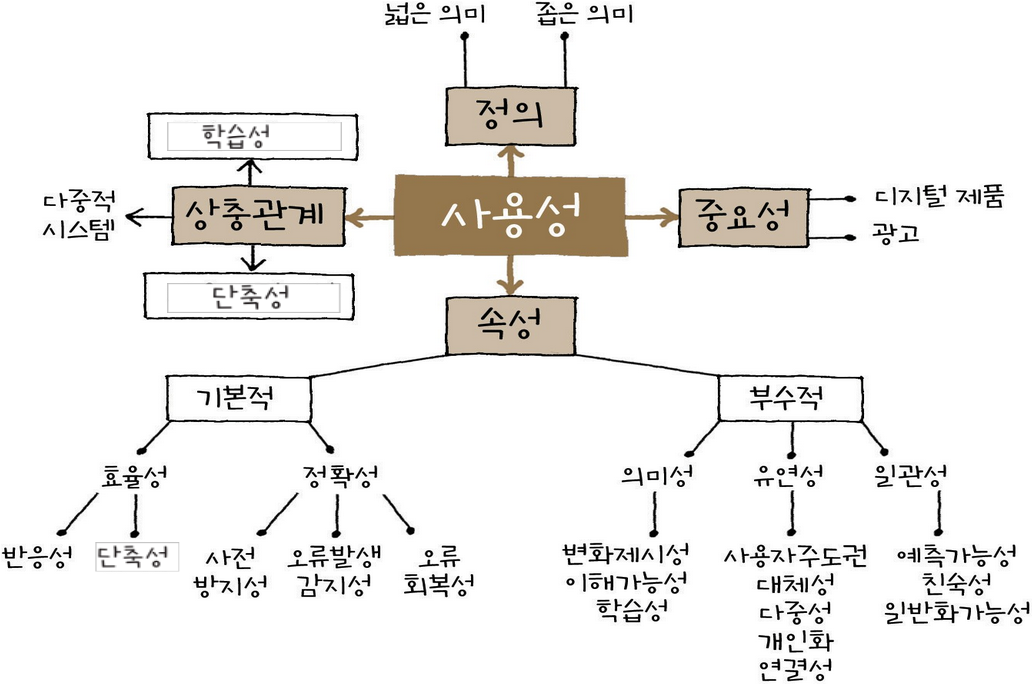
\includegraphics[width=\columnwidth,height=5cm]{usability.png} \end{figure}
\vspace{-3mm}

\bitmz
  \itm 사용성: 목표하는 기능을 수행하는 과정이 얼마나 효율적인가? 넓은 의미로는 시스템을 통해 과업을 수행하는 과정에서 사용자가 느끼는 총제적인 품질.
  \itm 효율성 차원: 반응성(속도), 단축성.
  \itm 정확성 차원: 사전방지성(오류 발생 가능성을 미연에 제거하거나 줄임으로써 사용자가 실수하는 것을 사전에 방지하는 속성, 사전 경고 및 심사), 오류 발생 감지성(사용자가 가능한 빨리 오류가 발생했다는 사실을 인식하고 조치를 취할 수 있어야, 잔상효과 및 시청각 알림), 오류회복성(시스템이 사용자로 하여금 오류를 정정할 수 있게 해야, 후방 오류 회복: 오류의 효과를 취소하고 오류 발생 이전 상태로 되돌림, 전방 오류 회복: 이전 상태로 돌아가는 대신 오류를 감수하고 다음 상태로 진행.)
  \itm 의미성 차원: 사용자가 관심있는 정보를 제공해야, 변화제시성(상태 변화를 사용자가 감지할 수 있어야, 즉시성 및 부가성), 이해가능성(전달된 정보를 사용자가 이해할 수 있어야, 가독성 및 논리성), 학습성(사용자가 쉽게 지식을 취득할 수 있어야, 매뉴얼, 적합성, 기억가능성).
  \itm 유연성 차원: 사용자가 원하는 작업을 시스템을 통해 원하는 방식으로 수행할 수 있어야, 사용자 주도권(모드 최소화, 사용자와 시스템이 통제권을 유연하게 주고받는 과업 전이성), 대체성, 다중성(동시성), 개인화, 연결성(연동성, 호환성).
  \itm 일관성 차원: 시스템의 정보나 기능이 다른 대상과 비슷한 모습 또는 역할을 가지는가?
\eitmz

\sectiondense{Game Design}

\bitmz
  \itm 라프 코스터의 재미이론: 재미(어떤 문제를 정신적으로 해결했을 때 느끼는 즐거움), 심미적 감상(아름다운 것을 보거나 들었을 때 느끼는 즐거움), 본능적 반응(본능적인 반응 자체만으로는 즐겁지 않고, 도전을 성취했을 때 보상이 작동하면 즐거움), 사회적 위치(다른 사람과의 경쟁에서 느끼는 즐거움).
  \itm 게임 디자인의 핵심 요소: 코어 매커니즘, 스토리텔링과 내러티브, 인터랙티비티.
  \itm 게임성: 공정성(실력이 좋은 플레이어가 이길 가능성이 높아야. 단, 실력자가 무조건 이기는 것은 아님.), 다양한 도전이 필요(논리, 기억, 지능, 지식, 도덕).
  \itm 정적 밸런스: 공격력, 방어력 등 수치를 통한 밸런싱. Dominance strategy는 상대방의 전략과 상관없이 최선의 선택이 되는 전략.
  \itm 동적 밸런스: 컴퓨터와 대결 중 사람이 잘하면 그에 맞게 컴퓨터의 실력이 높아짐.
  \itm 네 종류의 플레이어가 적절한 비율일 때 게임이 성공한다: Killer(플레이어 지향, 행동 선호, 빡겜러), Socializers(플레이어 지향, 인터랙션 선호, 친목러), Achievers(월드 지향, 행동 선호), Explorers(월드지향, 인터랙션 선호, 월드를 돌아다니며 구경).
\eitmz

\sectiondense{User Analysis}

\bitmz
  \itm 개발자도 사용자라는 인식, 자신의 경험이 보편적이라는 착각.
  \itm 사람들은 스스로의 필요를 모름, 분석할 시간과 비용도 부족하기 때문에 어려움.
  \itm 주사용자: 실제로 시스템을 사용하는 사람. 직접 시스템과 상호작용. 주 사용자는 분석해야.
  \itm 부사용자: 주 사용자가 시스템을 사용하는데 영향을 주거나 받는 사람. 실사용하지 않는 구매자, 학부모나 매니저.
  \itm 사용자의 숙련도, 행태적 특성, 개인적 특성을 조사해야.
\eitmz

\sectiondense{Context Analysis}

\bitmz
  \itm 사용자가 어떤 환경에서 시스템을 사용하는지를 통칭해 컨텍스트라고 한다.
  \itm 사용맥락: 좁은 의미로는 환경에 대한 설명, 넓게는 환경과 사용자의 상호작용 행위.
  \itm 물리적 맥락: 사용자의 주관적 관념이 들어가지 않고 기계적으로 측정되는 맥락 요소. 시간, 위치, 조명, 온도, 소음.
  \itm 사회적 맥락: 사람과 사람간 관계적 내용을 파약해야 측정할 수 있는 맥락 요소. 시간(업무 시간과 여가 시간), 위치(집/직장, 프라이버시), 조직 계층, 표준, 권력.
  \itm 문화적 맥락: 한 집단에 속한 사람들을 다른 집단에 속한 사람들과 구분되게 하는 가치관. 시간(과거/미래 지향), 위치(권력 거리), 환경(불확실성 회피, 암시/명시)
\eitmz

\sectiondense{Task Analysis}

\bitmz
  \itm 과업 분석의 목표는 사용자의 목적과 의도를 파악하는 것. 시스템이 사용자의 의도와 목적에 부합하는 것은 유용성을 달성하기 위한 선결 조건.
  \itm 명시적 지식과 묵시적 지식: 사용자는 매뉴얼, 규정과 같은 명시적 지식에 따라 시스템을 사용하지 않음. 따라서 실제로 사용자가 어떻게 과업을 수행하는지 분석해야.
  \itm 계층적 과업 분석(하나의 작업을 큰 과업과 세부 과업으로 계층적 구분), 지식 기반 분석(과업을 수행하기 위해 필요한 도구와 행위에 대한 지식에 기반), 시나리오 기반 분석(시스템을 사용하는 사용자의 구체적인 경험을 순차적으로 기술), 시퀀스 모형 분석(세부적인 과업을 실행하는 과정을 순차적으로 기술, 결합 시퀀스 모형으로 여러 사용자에게 과업을 수행하게 하고 일관된 시퀀스를 분류할수도.), Job 분석(사용자가 일반적으로 하루나 한달을 보내는 방식을 분석), 작업흐름 분석(전체 일을 수행하는 과정에서 누가 어떤 일을 하고 이를 위해 어떤 기능이 필요한지 분석), 맥락질문법(실제 사용자를 인터뷰, 이를 바탕으로 시나리오 작성하고 시퀀스 모델을 통해 추상화.).
\eitmz

\sectiondense{Tech Analysis}

\bitmz
  \itm 무조건 최고의 기술을 선택하는게 아님. 시스템이 갖춰지지 않은 경우 사용자가 감당 가능한 상한이 없음. 따라서 즉시 파괴적 혁신이 가능.
  \itm 디지털 기술의 분류: 디지털 플랫폼(여러 컴포넌트로 구성된 통합 시스템), 디지털 컴포넌트(플랫폼을 이루는 단위 기술, 입출력 장치), 플랫폼은 능동적vs수동적, 도구적vs유희적, 개인용vs공유용. TV는 수동적+유희적+공유용.
\eitmz

\sectiondense{Concept Design}

\bitmz
  \itm 컨셉: 제품의 기술과 원리, 형태를 포함해 제품이 어떻게 고객의 요구를 만족시킬 것인지 설명한 개념. 시스템 디자인의 첫 단계.
  \itm 좋은 컨셉은: 무결성(외부적으로는 고객의 기대, 내부적으로는 사내 기술력, 제품 성능을 조화해 통합된 컨셉으로 도출), 차별성(기존 제품과 구분되는 차별화된 패러다임을 창출), 집중성(소비자의 잠재된 요구를 만족, 타겟층을 예측할 수 있도록 도움.)
  \itm 방법론: TRIZ, 디자인 씽킹 등.
  \itm 메타포: 어느 한 영역에 대한 이해를 통해 다른 영역을 이해하거나 경험하는 행위. 메타포는 원천 영역과 목표 영역을 연결한다. 사용자의 심성모형과 개발자의 심성모형을 동기화.
  \itm 표면적 메타포(원천 영역과 목표 영역간 표면적인 부분만 일치), 구조적 메타포(원천 영역과 목표 영역의 구성요소들이 일치), 합목적 메타포(대상을 사용하는 목적이 일치).
  \itm 메타포 선정 절차: 기능집합 만들기(페르소나, 과업 분석 등), 후보 메타포 파악, 메타포와 시스템 간의 일치도 분석, 주 메타포 선정, 보조 메타포 선정, 메타포 모형 작성.
\eitmz

\sectiondense{Information Design}

\bitmz
  \itm 정보구조 디자인: 데이터를 분류, 배열, 조직화해 질서를 부여. 사용자에게 필요한 데이터를 선정하고 사용자가 이해하기 쉽게 분류, 구조화한다.
  \itm 사용자가 시스템의 정보 구조를 탐색하는 것을 내비게이션이라고 함.
  \itm 정보구조 디자인 단계: (1) 사용자에게 의미있는 다양한 원자료를 수집, (2) 특정 기준에 따라 자료를 분류, (3) 정보 구조 결정, (4) 정보의 구조 사이를 이동하는 기본 방법(내비게이션 구조) 설정, (5) 내비게이션 지원 시스템을 디자인.
  \itm 정보의 유형: 사실, 개념, 절차, 원리, 원칙, 이야기, 의견, 묘사, 예측, 메타데이터.
  \itm 상향식 설계: 수집된 다양한 자료로부터 이들을 효과적으로 구분할 수 있는 기준을 도출. 제1기준: 객관적인 분류(글자, 위치, 시간 등, 상호배타적이고 정형화됨), 주관적인 분류(주제, 사용자 등). 제2기준: 정적인 분류, 동적인 분류(한 범주에 분류된 자료가 추후 다른 범주료 분류 가능).
  \itm 정보구조: 순차적, 그리드, 계층, 네트워크(웹, HTTP), 대중분류(위키), 그리고 이들을 혼합.
\eitmz

\sectiondense{Interaction Design}

\vspace{-3mm}
\begin{figure}[h] \centering 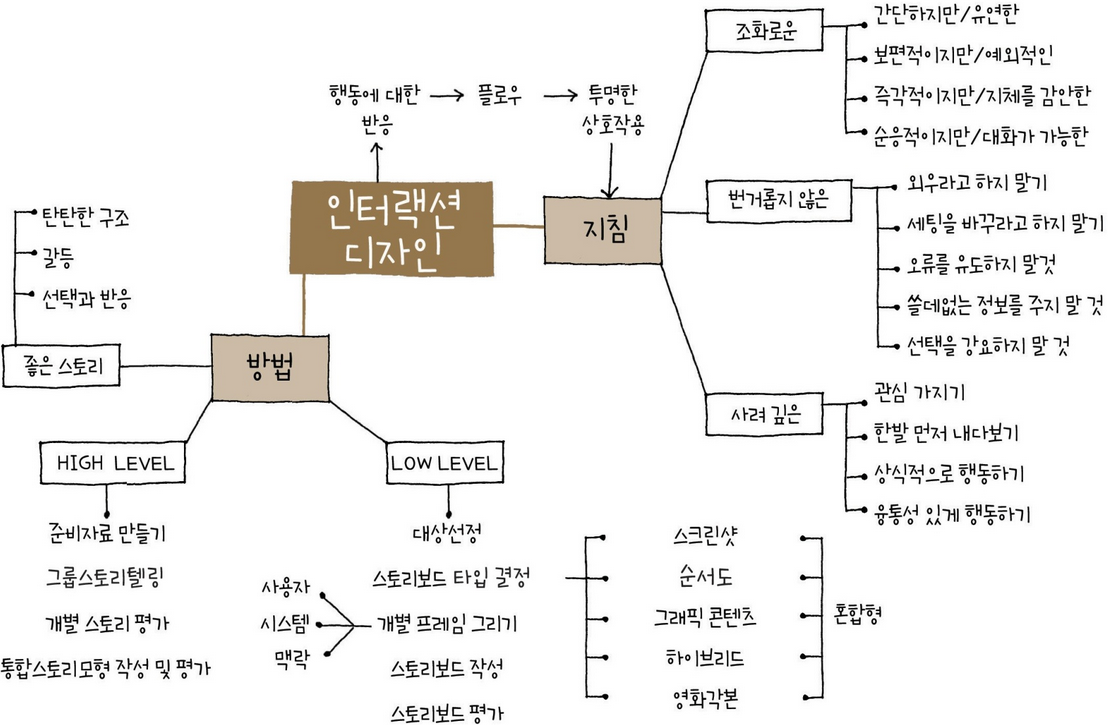
\includegraphics[width=\columnwidth,height=6cm]{interaction-design.png} \end{figure}
\vspace{-3mm}

\bitmz
  \itm 상호작용이란 사용자가 시스템과 커뮤니케이션하는 모든 과정.
  \itm Flow: 몰입, flow 상태에 돌입하면 생산성이 높아진다. 투명한 인터랙션은 flow를 만든다. 사람이 시스템을 통해 과업을 달성하고자 할 때, 시스템이라는 기계적 요소가 사람에게 느껴지지 않아서 사람이 자신의 목적을 직접 달성하고 있다고 생각하게 만드는 것을 투명성이라고 함. 투명한 DX를 위해서는 과업을 조화롭게 수행, 불필요한 행동 최소화, 불편에 대해 사려 깊게 행동해야.
  \itm 조화로운 인터랙션을 위한 4원칙: 간단하지만 유연한 인터랙션, 보편적이지만 예외적인 상황을 고려한 인터랙션, 즉각적이지만 지체를 감안한 인터랙션, 순응적이지만 대화가 가능한 인터랙션.
  \itm 부정적 요소를 줄이기 위한 지침: 암기를 요구하지 말라, 세팅을 변경하도록 강요하지 말라, 오류를 범하게 유도하지 말라, 불필요한 정보를 받게 하지 말라, 선택을 강요하지 말라.
  \itm 긍정적 요소를 증진하기 위한 지침: 사용자에게 관심을 가져야, 한 발 먼저 내다봐야, 상식적으로 행동해야, 유연하게 반응해야.
  \itm 스토리보드 기법: 사용자와 시스템 사이 인터랙션을 중심으로, 사용자가 시스템을 사용하는 스토리를 그래픽으로 표현하는 방법. 전반적인 스토리 구축(자료 준비, 그룹 스토리텔링-개별 스토리 평가-통합 스토리 모형-통합 스토리 모형 평가 및 수정 보완)
\eitmz

\sectiondense{Interface Design}

\vspace{-3mm}
\begin{figure}[h] \centering 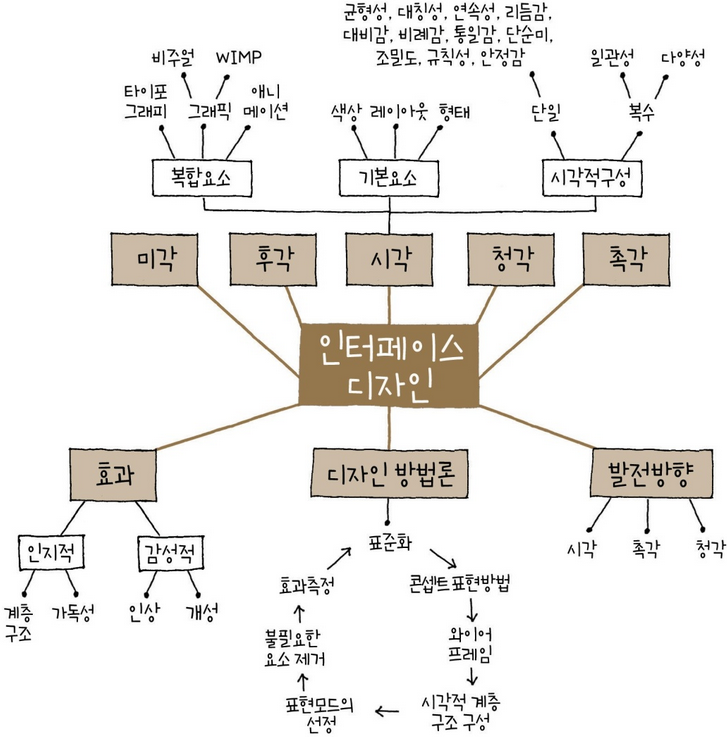
\includegraphics[width=\columnwidth,height=6cm]{interface-design.png} \end{figure}
\vspace{-3mm}

\bitmz
  \itm 기본적인 시각 디자인 요소: 색(색상, 명도, 채도, 톤), 모양(크기, 방위, 형태), 레이아웃(정보의 양, 그룹, 정렬, 정보간 공간적 관계), 타이포그래피, 그래픽(이미지, 다이어그램, 표 등), 애니메이션.
  \itm WIMP 4요소: 윈도우, 포인터(커서), 메뉴, 아이콘(ISO 표준이 있음).
  \itm 균형성(시각적 무게), 대칭성, 연속성(자연스러운 시선의 흐름), 리듬감, 대비감, 비례감, 통일감, 단순미, 조밀도, 규칙성, 안정감, 일관성(적응성 및 예측 가능성), 다양성.
  \itm 인터페이스 디자인의 효과:
  \bitmz
    \itm 유용성 측면 효과: 시각적 계층 구조(한 페이지 안의 구성 요소의 위치와 관계를 성정함으로써 사용자가 구성 요소를 단계적으로 인지할 수 있음)를 이루는 화면 구성. e.g., 대비, 전경과 배경의 구분, 기능별 배치, 색상과 톤을 이용한 계층 구조 형성 등.
    \itm 사용성 측면의 효과: 가독성. 색상과 폰트, 배치 등.
    \itm 감성 측면의 효과: 미적 인상(외부 자극으로 각인되긴 했지만, 정서로 관념화되지 않은 감성) 및 개성.
  \eitmz
  \itm 인터페이스 디자인 절차:
  \bitmz
    \itm 메타포 표현: 제품의 컨셉을 확립, 전체적인 메타포를 설정.
    \itm 정보 구조 표현: 와이어프레임 설계.
    \itm 시각적 구조 표현: 내용간 시각적인 계층구조를 구성.
    \itm 다양한 모드 활용: 사용자와 환경에 따라 다양한 모드를 제공하도록 고도화.
    \itm 불필요한 요소 제거: 불필요한 요소를 제거.
    \itm 디자인 효과 측정: 내외부적으로 피드백을 받고 평가.
    \itm 추상화 표준화: 일관된 인터페이스 시스템을 확정, 디자인 시스템 설계.
  \eitmz
  \itm 인터페이스 디자인은 시스템과 관련된 모든 요소에 대한 표현 방법을 정하는 단계. 시각적 디자인 요소(색, 모양과 같은 기본적 요소, 타이포그라피와 같은 복합적 요소, 기본 요소들의 집합으로 표현되는 시각적 구성)를 가장 많이 사용하며, 이를 통해 여러 효과(시각적 계층 구조, 가독성, 미적인상)를 얻을 수 있음.
\eitmz

\sectiondense{UX Evaluation \& Innovation}

\bitmz
  \itm 평가 목적에 따라: 결론적 평가(특정 기준을 미리 세워놓고 서비스가 기준을 최종적으로 통과했는지 평가), 탐험적 평가(여러 대안을 생각해보고 그 중 각 대안의 장단점이 무엇인지 파악하기 위한 평가), 진화적 평가(시스템을 개발하는 단계에 맞춰 결론적 평가와 탐험적 평가를 적절히 배합하는 평가)
  \itm 오즈의 마법사: 시스템이 실제로 작동하는 것처럼 보이지만, 백엔드에서는 개발자가 수동으로 사용자의 행동에 대응하는 프로토타입. (스케치-스냅-선택-연결-실행)
  \itm 분석적 평가: 실제 사용자를 참여시키지 않고 시스템을 평가. 휴리스틱 검사(소수의 전문가들이 부분적으로 검사), 리스트 검사, 리허설 검사, 모형 분석, 시뮬레이션.
  \itm 실증적 평가: 실제 사용자를 대상으로 시스템을 평가.
\eitmz
